\begin{figure}[ht!]
	\caption{Diagram of what happens when Alice turns.}
	\label{fig:turningAlice}
	\centering
	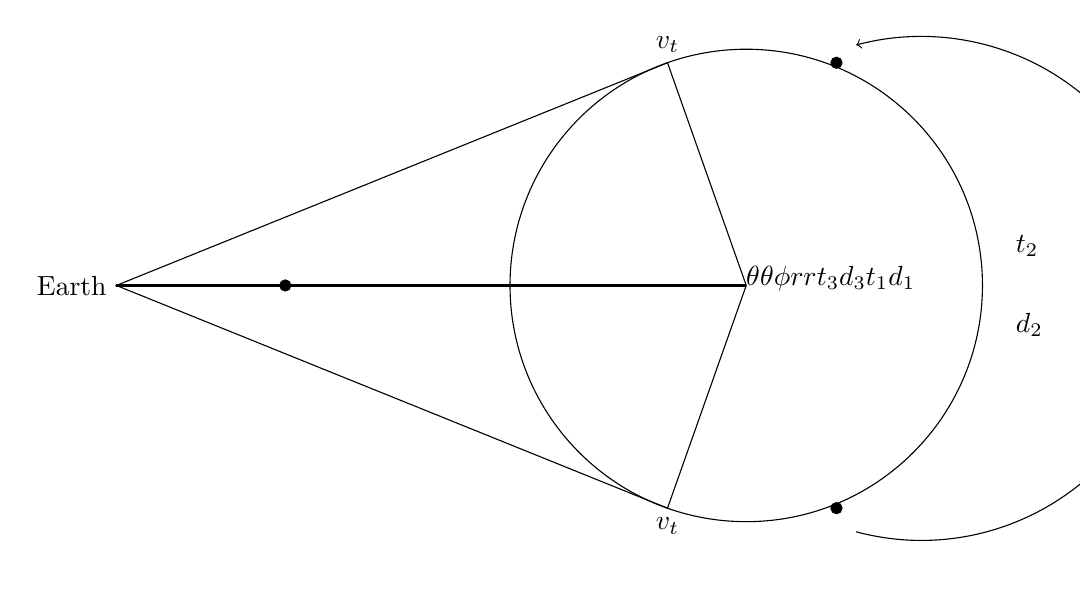
\begin{tikzpicture}
		\coordinate (O) at (0,0);
		\coordinate [label=left:Earth] (E) at (-8,0);
		\coordinate [label=above:$v_t$] (A) at (-1,2.828427125);
		\coordinate [label=below:$v_t$] (B) at (-1,-2.828427125);
		\coordinate [label=right:$\Del t_2$] (T) at (3.3,0.5);
		\coordinate [label=right:$\Del d_2$](D) at (3.3,-0.5);

		\draw (O) circle (3);
		\draw (A) -- (O) -- (B) -- (E) -- cycle;
		\draw[thick](O) -- (E);

		\tkzMarkRightAngle(E,A,O);
		\tkzMarkRightAngle(E,B,O);

		\tkzMarkAngle[size=0.6](A,O,E);
		\tkzLabelAngle(A,O,E){$\theta$};

		\tkzMarkAngle[size=0.6](E,O,B);
		\tkzLabelAngle[pos=-1](E,O,B){$\theta$};

		\tkzMarkAngle[size=0.75](B,O,A);
		\tkzLabelAngle(B,O,A){$\phi$};

		\tkzLabelSegment[above right](O,A){$r$};
		\tkzLabelSegment[below right](O,B){$r$};

		\tkzLabelSegment[above=1.25em](E,A){$\Del t_3$};
		\tkzLabelSegment[above=0.25em](E,A){$\Del d_3$};

		\tkzLabelSegment[below=0.25em](E,B){$\Del t_1$};
		\tkzLabelSegment[below=1.25em](E,B){$\Del d_1$};

		\draw[->] (-0.75,-3.128427125) arc (-105:105:3.2);

		\filldraw[black] (A) circle (2pt);
		\filldraw[black] (B) circle (2pt);
		\filldraw[black] (E) circle (2pt);
	\end{tikzpicture}
\end{figure}
